%!TEX root = ../main.tex

\section{Introduction}
\label{s:intro}
% \ewu{we really need to emphasize that this is a HARD problem!!}

Poor data quality is a hard and persistent problem.  It is estimated to cost the US economy more than \$600 billion
per year~\cite{eckerson2002} and erroneous price data in retail databases
alone cost the US consumers \$2.5 billion each year~\cite{Fan2008}. Although data
cleaning tools can purge many errors from a dataset before downstream 
applications use the data, databases are constantly changing as applications
and users execute queries that modify the data.
Mistakes in these queries can introduce errors that spread through the database
due to subsequent update queries; 
by the time errors are detected, it is difficult to trace those errors back to the 
erroneous query and correct it.
Identifying and correcting errors in the data directly is suboptimal: it treats the symptom,
rather than the underlying cause. Fixing the manifested data errors on a
case-by-case basis often obscures the root of the problem and other data that may have been
affected. Therefore, traditional data cleaning approaches are not well-suited
for this setting: While they provide general-purpose tools to identify and
rectify anomalies in the data, they are not designed to diagnose the causes of
errors that are rooted in erroneous updates.
Some data cleaning systems try to identify structural sources of
mistakes~\cite{wang2015}, but they are unable to trace the source of
the mistakes to particular faulty queries.

While improving data quality and correcting data errors has been an important
focus for data management research, handling new errors, introduced during
regular database interactions, has received little attention. Most work in
this direction focuses on \emph{guarding against} erroneous updates. For
example, integrity constraints~\cite{Khoussainova2006} reject some improper
updates, but only if the data falls outside rigid, predefined ranges.
Certificate-based verification~\cite{Chen2011} is less rigid, but it is
impractical and non-scalable as it requires users to answer challenge
questions before allowing the updates, and it is not applicable to updates
initiated by applications.


In this demo proposal, we outline the design of \sys, a framework that derives explanations
and repairs for discrepancies in relational data based on potential errors in
the queries that operated on the data, and describe how users will use \sys
in a demonstration scenario. 
In contrast to existing approaches in data
cleaning that aim to detect and correct errors in the data directly, the goal
of \sys is to identify errors in the queries that introduced errors in the
data. These diagnoses both \emph{explain} how errors were introduced to a
dataset, and also lead to the identification of additional discrepancies in
the data that would have otherwise remained undetected.
Participants will be able to select from a number of 
transactional benchmarks, introduce errors into the queries that are executed,
and compare the fixes to the queries proposed by \sys as well as existing alternative algorithms
such as decision trees.



% \begin{example}[Wireless discount policies]\label{ex:telco}
% 
% A large US-based wireless provider offers company discounts as incentives for
% corporate customers. There are different types of discounts (flat, percentage,
% fee-based), and their details are specific to corporate agreements. The large
% number of policies and complexities in their rules frequently cause policies
% to be set incorrectly, leading to errors in the application of discounts to
% customers' accounts.
% 
% Customers who notice billing errors contact the provider, but the call centers
% do not have the capacity or ability to investigate the complaints deeply. The
% standard course of action is to correct billing mistakes on a case-by-case
% basis for each complaint. As a result, unreported errors remain in the
% database for a long time, or they never get corrected, and their cause becomes
% harder to trace as the source of the errors is obscured.\footnote{This is a real-life scenario, provided to us by a popular US-based wireless provider.}
% 
% \end{example}

\begin{example}[Tax bracket adjustment]\label{ex:taxes}
    
Tax brackets, which determine tax rates for different income levels, are
often adjusted. Accounting firms implement these changes to their
databases by appropriately updating the tax rates of their customers. Mistakes
in these update queries (e.g., Figure~\ref{fig:example}) result in errors in
the tax rates and computed taxes. 

\end{example}


In this application, data errors are typically reported to a
customer service department, which does not have the resources nor the
capability to investigate the errors more broadly. Instead, errors are
resolved on a case-by-case basis. In practice, customer service only deals
with a small portion of the actual errors. Once these errors are resolved,
there will still be a large number of incorrect records that were not
identified. The goal of \sys is to identify the query or queries that caused
the errors, propose corrections to those queries, and use the modified queries
to identify other errors.

Diagnosing data errors stemming from incorrect updates is fundamentally
challenging: the search space of possible mistakes and fixes is large, and the
amount of information (number of known errors) may be limited. The problem has
the following important characteristics that render traditional data cleaning
methods unsuitable:



\begin{description}[leftmargin=*, topsep=0mm, itemsep=0mm]
    
    \item[Obscurity.] Detection of the resulting errors in the data often
    leads to partial fixes that further complicate the eventual diagnosis and
    resolution of the problem. For example, a transaction implementing a
    change in the state tax law updated tax rates using the wrong rate,
    affecting a large number of consumers. This causes a large number of
    complaints to a call center, but each customer agent usually fixes each
    problem individually, which ends up obscuring the source of the problem.
    
    \item[Large impact.] Erroneous queries cause errors at a large scale. The
    potential impact of the errors is high, as manifested in several
    real-world cases~\cite{Yates10, Grady13, sakalerrors}. Further, errors
    that remain undetected for a significant amount of time can instigate
    additional errors, even through valid updates. This increases both their
    impact, and their obscurity.
    
    \item[Systemic errors.] The errors created by bad queries are
    \emph{systemic}: they have common characteristics, as they share the same
    cause. The link between the resulting data errors is the query that
    created them; cleaning techniques should leverage this connection to
    diagnose and fix the problem. Diagnosing the cause of the errors, will
    achieve systematic fixes that will correct all relevant errors, even if
    they have not been explicitly identified.
    
\end{description}
% 
\sys addresses these challenges by analyzing the queries that operated on a
dataset in an efficient and scalable manner. More concretely, we make the
following contributions:


% The goal of this paper is to design effective query
% diagnosis techniques and identify possible fixes for query errors. We
% model the problem assuming a log of update workloads over a database,
% and a set of complaints that identify errors in the final database
% state. We organize our contributions as follows:

% \ewu{really like this organization}

% \ewu{add: special case optimizations for single query case.}


% \begin{itemize}[leftmargin=*, topsep=0mm, itemsep=0mm]      
%     \item We formalize the problem of diagnosing a set of errors using log
%     histories of updates that operated on the data. Given a set of 
%     \emph{complaints} as representations of data discrepancies in the current
%     state of a dataset, \sys identifies the queries in the log that require the  minimal
%     amount of changes that would resolve all of the complaints (Section~\ref{sec:abstractions}).
%       
%     \item We provide an exact error-diagnosis solution through a non-trivial
%     transformation of the problem to a mixed integer linear program (MILP) that
%     encodes the data provenance of the erroneous tuples. Our approach employs state-of-the-art MILP solvers to identify
%     optimal diagnoses that are guaranteed to resolve all complaints without introducing new errors to the data
%     (Section~\ref{sec:sol}).
%     
%     \item We present several optimizations to our basic diagnostic
%     method, which reduce the problem size without affecting the
%     quality of the produced solutions. Further, we propose an
%     incremental repair method that targets the cases where the log
%     contains a single corrupted query (or the search focuses on a
%     single repair). This incremental analysis of the log allows us to
%     scale to very large datasets and large query logs. Further, we
%     show that our optimization techniques have the additional
%     advantage of tolerating incomplete information, such as unreported
%     errors (Section~\ref{sec:opt}).
% 
%     
%     % \item We extend our framework to also handle false positives: complaints
%     % that mistakenly identify data as erroneous. We define the notion of
%     % complaint \emph{density}, which is a query-driven measure of closeness of
%     % a complaint to other complaints. The main intuition of our approach is
%     % that complaints of low density are likely false positives and thus can be
%     % safely ignored (Section~\ref{???}).
%     
%     \item We experimentally evaluate the effectiveness and efficiency of our
%     methods against real-world and synthetic datasets and query logs. 
%     (Section~\ref{sec:experiments}). 
% \end{itemize}



\section{{\large\textbf{\sys}}: architecture}


\begin{figure}[t]
    \centering
        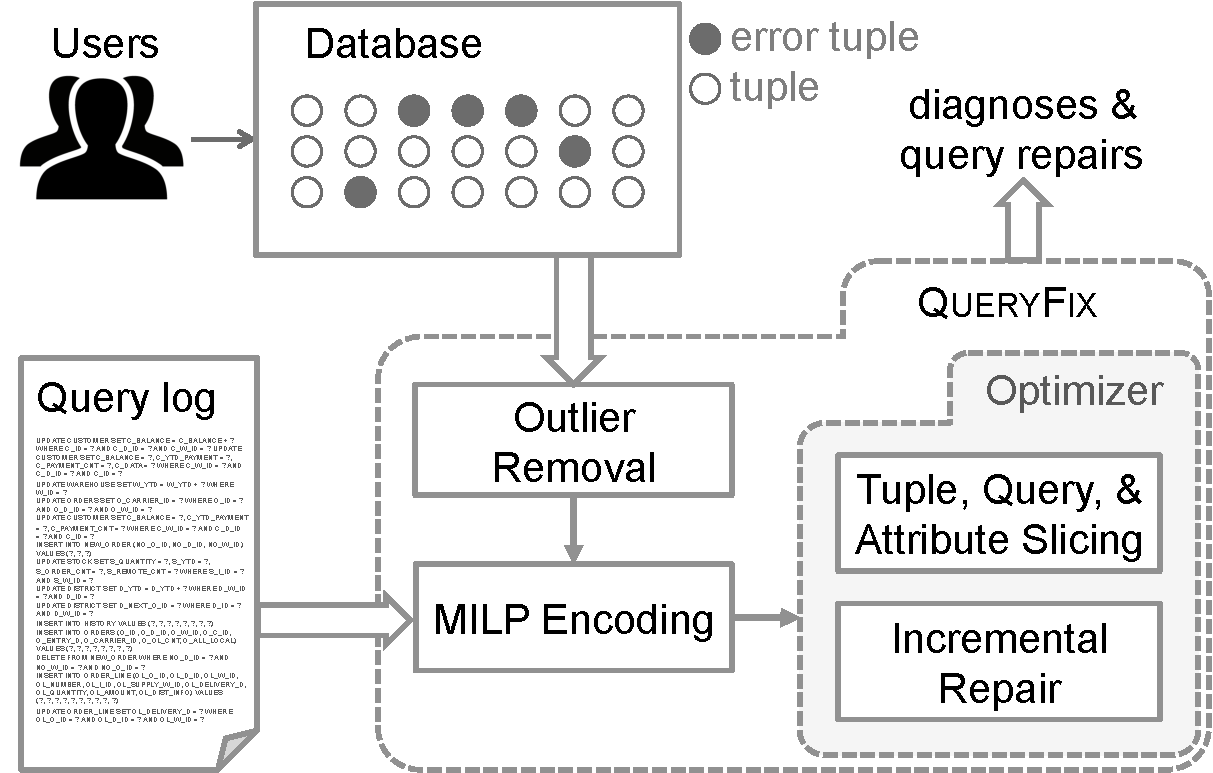
\includegraphics[scale=0.40]{figures/architecture}
    \caption{\sys processes data anomalies in the form of complaints and analyzes logged query histories to identify the causes of error. In the heart of the system, transformation algorithms express the diagnosis problem as a mixed integer program, and optimization modules ensure that the MIP programs can be evaluated efficiently.}
    \label{fig:architecture}
\end{figure}

Figure~\ref{fig:architecture} shows the architecture of \sys. The system uses
two inputs: a log of update queries (including UPDATE, INSERT, and DELETE
statements) and a set of identified data errors (\emph{complaints}). \sys
analyzes the data errors and the query logs to trace the causes of the errors
in queries in the log (diagnoses), and to automatically derive query repairs.
The query repairs represent corrections to the queries in the log, and can be
used to identify additional errors in the data that were not reported.

The core of \sys is a transformation module that expresses the query diagnosis
problem as a Mixed Integer Linear Program (MILP). Two performance optimization modules
ensure that the system can scale to large datasets efficiently, while
maintaining high accuracy. 


